\documentclass[12pt]{article}

\usepackage[margin=1in]{geometry}
	%changes default margins

\usepackage{setspace}
\usepackage{multirow}
\usepackage{booktabs}
\doublespacing
	%\singlespacing,\onehalfspacing,\doublespacing can be set and everything thereafter will use that spacing. You can switch within the document as often as you wish
	
\usepackage{parskip}
%changes paragraphs to have an extra space and new indentation with paragraphs, rather than indenting every new paragraph. This is completely a stylistic choice and neither is better than the other.


\usepackage{mathtools,amssymb} %useful math stuff. there are a lot of ams* packages. If you have a math need, it's probably in there

	
	
%\usepackage{natbib}
%\usepackage{biblatex} %natbib is older and available from almost all journals, biblatex is not, but biblatex has more flexibility and options.

%\usepackage[natbib=true]{biblatex} %this often works and requires minimal changes 

%for biblatex you write \textcite{citekey} and \parencite{citekey}
%for natbib you write \citet{citekey} and \citep{citekey}. Please avoid using \cite{} since you won't control whether it's parenthetical, but you are responsible for whether you use something in text or parenthetically.
%for \usepackage[natbib=true]{biblatex} you follow the natbib style and you won't have to perform search/replaces in your document, you would only need to change the package call and bibliography call.

\usepackage{natbib}
\bibliographystyle{chicago}

%other useful packages
% \usepackage{graphicx} %for including images including pdf



\title{Ast2: The Dark Forest}
\author{jsp ci 843503,\\ 
	eswst i; ,i;l 830097,\\ 
sjsms ,ovjs; 839866}
\date{\today}

\begin{document}
	
\maketitle

\section{Part 1: Electricity consumption}

\begin{enumerate}
	\item We use the daily mean temperature as the outside temperature measurement for this investigation.
	\item Using the following linear regression model:
\[
\mathbf{y}_{econ} = \beta_1 \mathbf{x}_{temp} + \beta_0 + \mathbf{\epsilon}
\] 
Where $\mathbf{x}_{temp}$ is the outside temperature (in °C), $\mathbf{y}_{econ}$ is the electricity consumption (in kWh) and $\mathbf{\epsilon}$ is the residual. After regression, we got $\beta_0 = 15.42925$ and $\beta_1 = -0.19582$, which yields the following equation:
\[
\hat{\mathbf{y}}_{econ} = -0.19582 \mathbf{x}_{temp} + 15.42925
\] 
Based on the given data and regression, we concluded that: 
The electricity consumption would decrease when the outside temperature increases.
\item The point estimates for the average electricity consumption are given in Table~\ref{Tab:1}.

\begin{table}[htpb]
	\centering
	\begin{tabular}{cccccc}
		\toprule
		\multirow{2}{*}{} &
		\multicolumn{5}{c}{Temperature $(^{\circ}\text{C})$}\\
		%\cline{2-6}
		 & -40 & -20 & 0 & 20 & 40 \\
		\midrule
		$\hat{\mathbf{y}}_{econ}$ (kWh)&23.27&19.35&15.43&11.51&7.59\\
		\bottomrule
	\end{tabular}
	\caption{The point estimate for the average electricity consumption with respect to the temperature. (simple linear regression model)}
	\label{Tab:1}
\end{table}
\item The plot of the data is shown in Figure~\ref{Fig:1}.
The scatter plot reveals a concave pattern indicating strong non-linearity: electricity consumption initially decreases with rising temperature, but increses again after the temperature rises to approximately 10 $^{\circ}$C.
\begin{figure}[htbp]
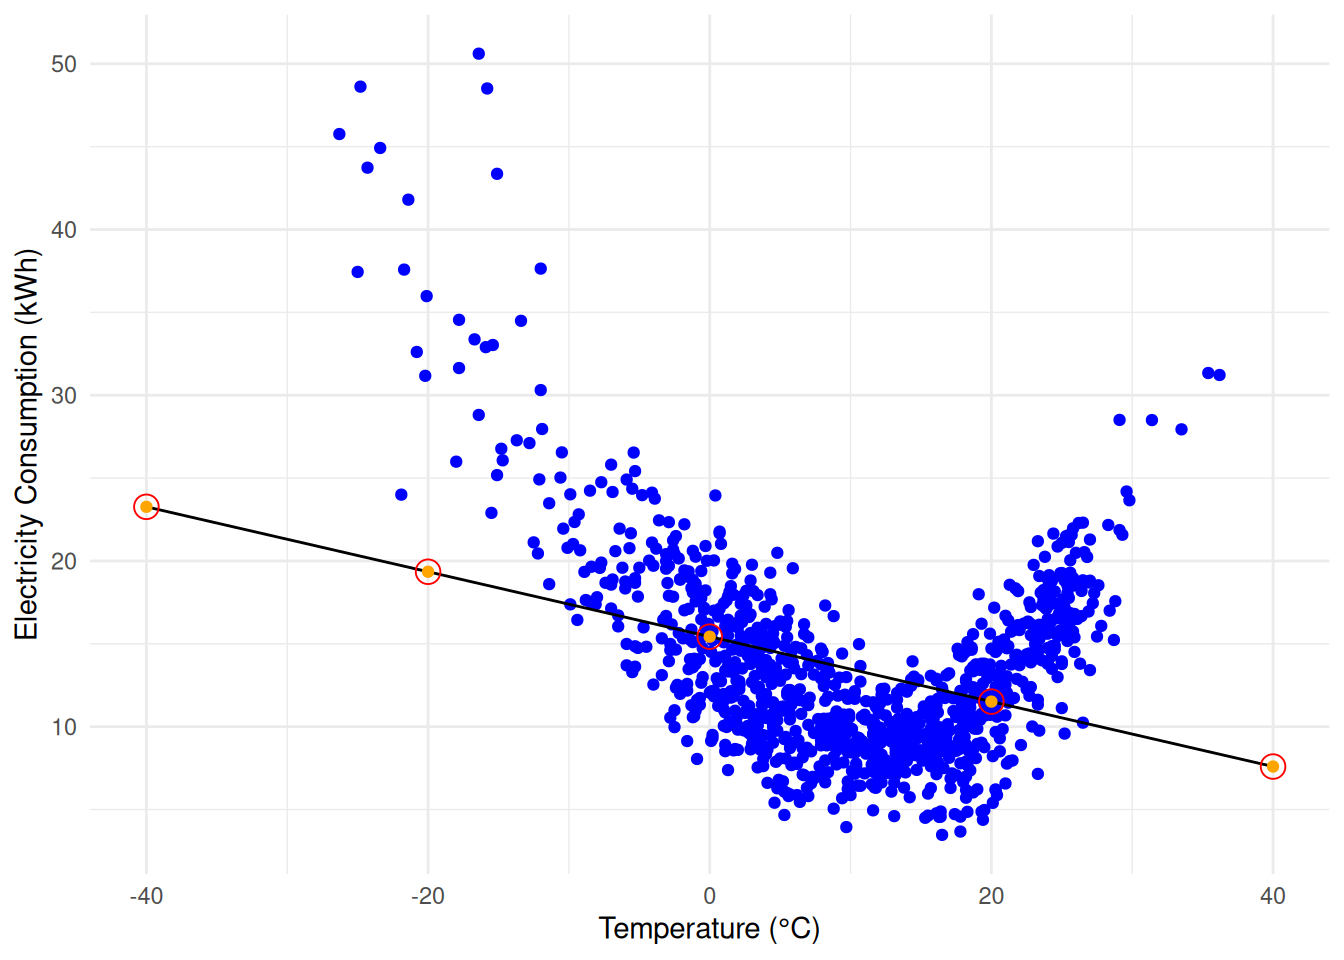
\includegraphics[width=.7\textwidth]{1.png}
\centering
\caption{Electricity consumption under different temperature with simple linear regression.}
\label{Fig:1}
\end{figure}
\item We added a quadratic term to the previous model, creating a new polynomial regression model:
\[
\mathbf{y}_{econ} = \beta_2 \mathbf{x}_{temp}^{2}
+\beta_1 \mathbf{x}_{temp} + \beta_0 + \mathbf{\epsilon}
\] 

After regression, we got $\beta_0 = 13.77471$, $\beta_1 = -0.65656$, and $\beta_2 = 0.02942$.

The axis of symmetry of the parabola is: $x_{temp} =  -\frac{\beta_1}{2\beta_2} = 11.15814$.

So, when the outside temperature is below 11.15814 $^{\circ}$C, the average electricity consumption of the resident decreases when the outside temperature rises; when the outside temperature is above 11.15814$^{\circ}$C, the resident uses more elctricity on average when the outside temperature rises.

\item The point estimate under the new polynomial regression model for the average electricity consumption is given in Table~\ref{Tab:2}.
The polynomial regression provides a better estimates than simple linear regression model.

\begin{table}[htpb]
	\centering
	\begin{tabular}{cccccc}
		\toprule
		\multirow{2}{*}{} &
		\multicolumn{5}{c}{Temperature $(^{\circ}\text{C})$}\\
		%\cline{2-6}
		 & -40 & -20 & 0 & 20 & 40 \\
		\midrule
		$\hat{\mathbf{y}}_{econ}$ (kWh)&87.11&38.67&13.77&12.41&34.59\\
		\bottomrule
	\end{tabular}
	\caption{The point estimate for the average electricity consumption with respect to the temperature. (polynomial regression model)}
	\label{Tab:2}
\end{table}

\item Figure~\ref{Fig:2} gives the scatter plot of the data and overlays the fitted polynomial regression curve. The five estimated values are plotted in orange dots and encircled in red. The model fit is better because the parabola captures the ``concave'' pattern of the data.

\begin{figure}[htbp]
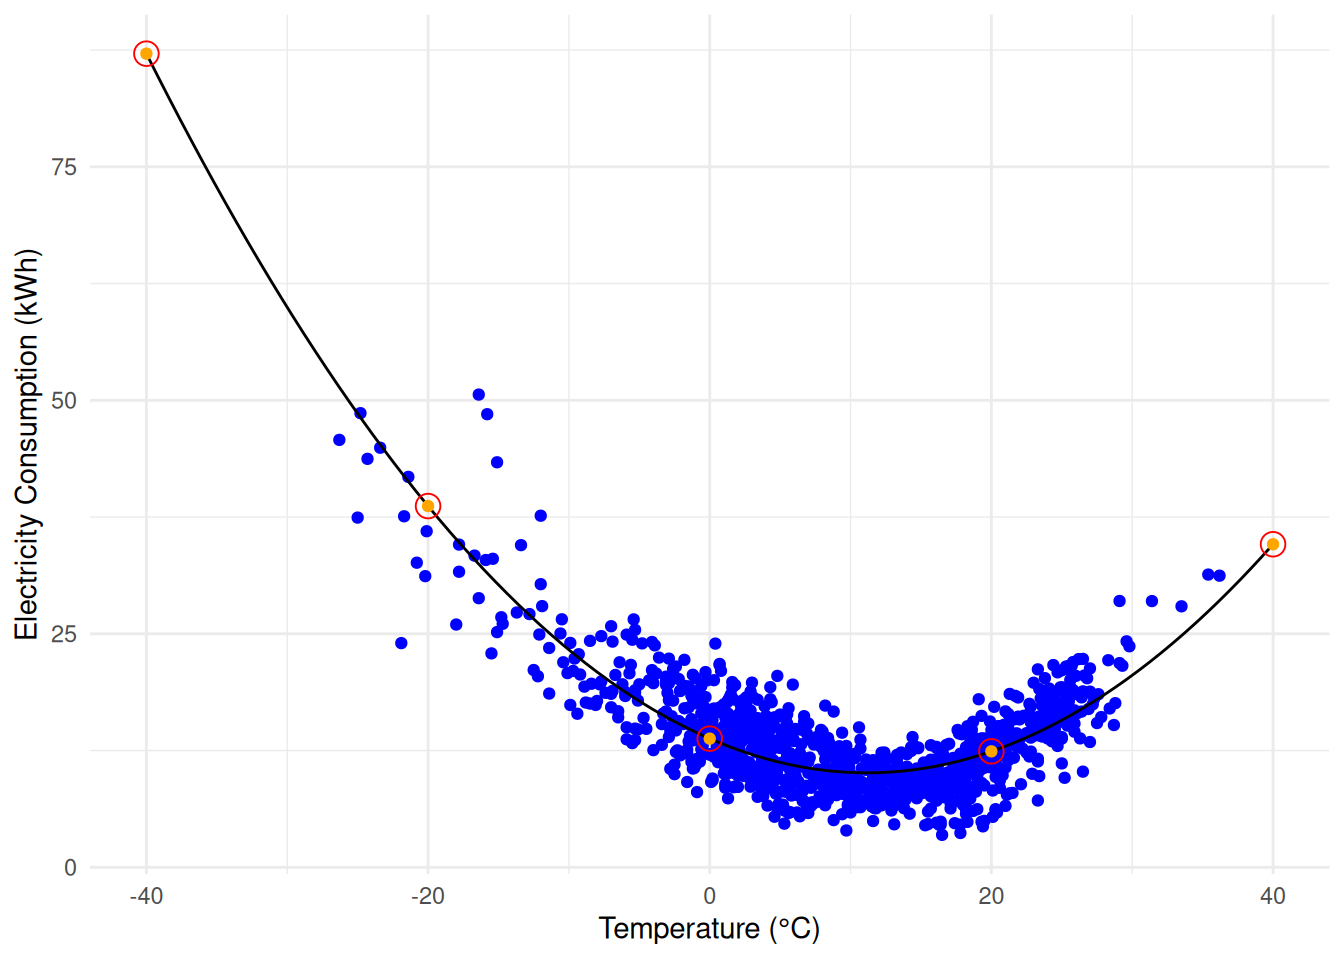
\includegraphics[width=.7\textwidth]{2.png}
\centering
\caption{Electricity consumption under different temperature with polynomial regression.}
\label{Fig:2}
\end{figure}
\end{enumerate}


\section{Part 2: Bushes data}
	
\begin{enumerate}

\item Simple linear regression model for bushes height and width:
\[
\mathbf{y}_{h} = \beta_1\mathbf{x}_w + \beta_0 + \mathbf{\epsilon} ,\] 
where $\mathbf{y}_h$ represents the height of plants, $\mathbf{x}_w$ represents the width of plants and $\mathbf{\epsilon}$ represents the residuals. After regression, we got the following regression line equation:
\[
\hat{ \mathbf{y} }_{h} = -0.8159\mathbf{x}_w + 6.7939
.\] 
The plot is shown in Figure~\ref{Fig:3}. The regression line captures the pattern that the average height of bushes (ignoring species) decreases when width increases. The slope of -0.8159 means the height of plants will decrease by 0.8159 in. if the width increases 1 in. For this regression model, $p < .001$ so it is significant.

\begin{figure}[htbp]
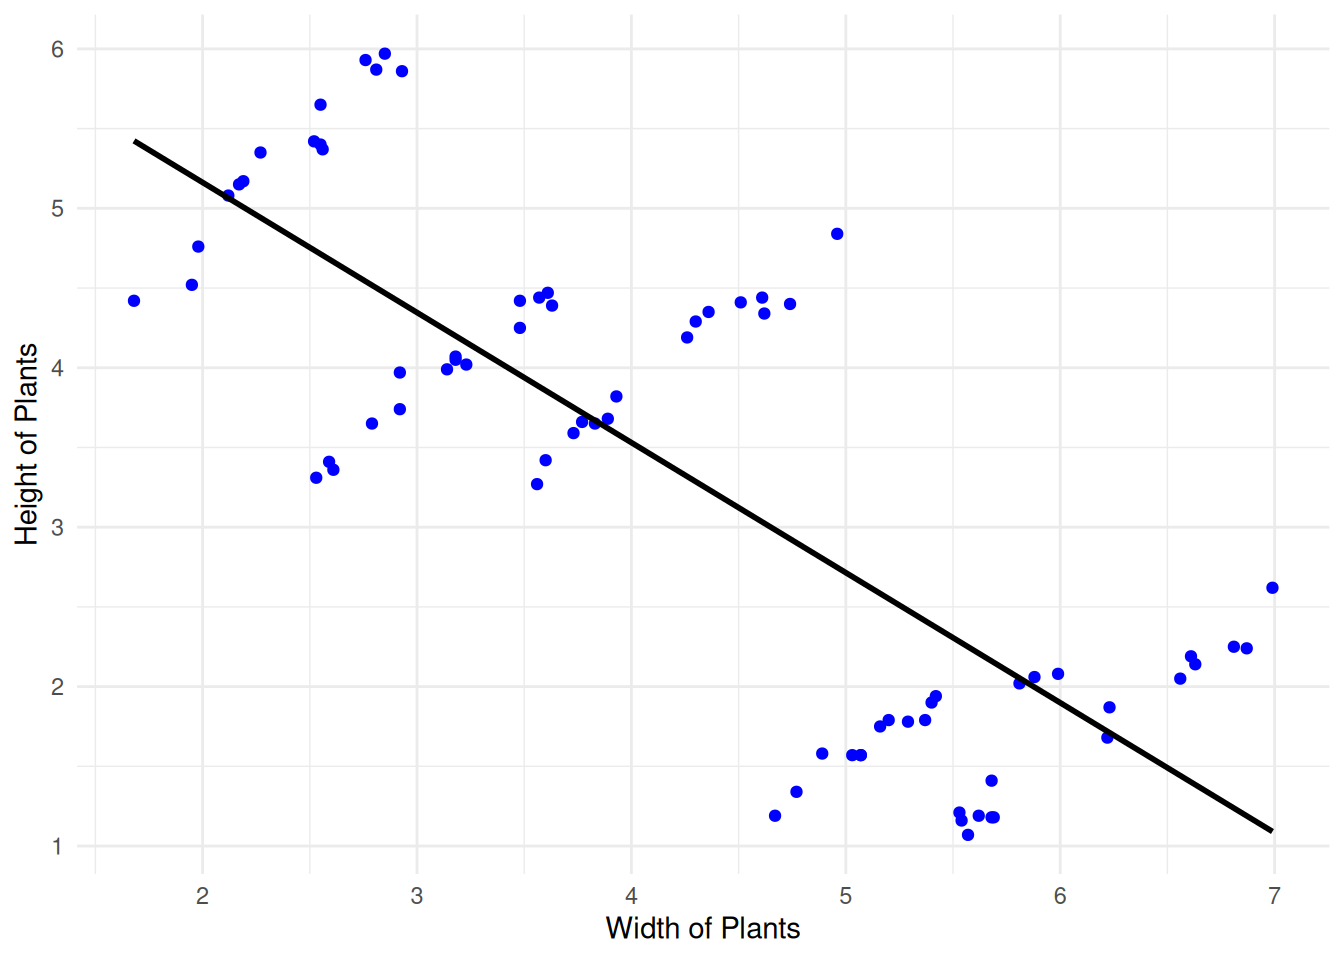
\includegraphics[width=.7\textwidth]{3.png}
\centering
\caption{Simple linear regression line of $\mathbf{y}_h \sim \mathbf{x}_w$ ignoring species.}
\label{Fig:3}
\end{figure}

\item Figure~\ref{Fig:4} shows the linear regression lines when {\em not} ignoring species. We can see 5 regression lines overlaying each of the 5 species.

\begin{figure}[htbp]
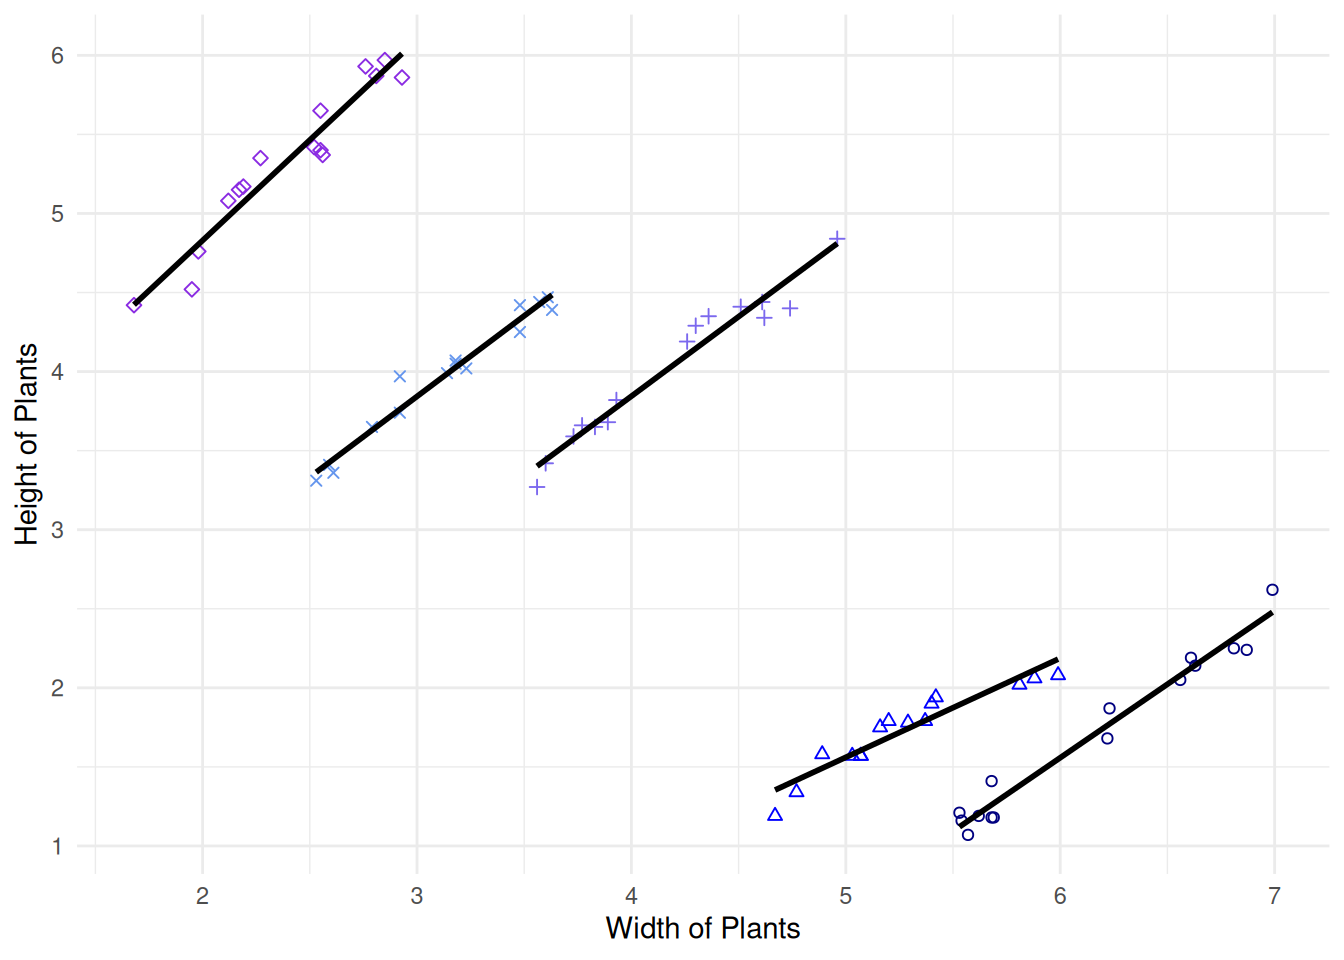
\includegraphics[width=.7\textwidth]{4.png}
\centering
\caption{Simple linear regression line of $\mathbf{y}_h \sim \mathbf{x}_w$ {\em not }ignoring species.}
\label{Fig:4}
\end{figure}

\item The slopes and $p$ values of the linear regression lines are shown in Table~\ref{Tab:3}. All slopes are positive, meaning that fixing the species, the average height of the plant increases when the width increases. Also we can see that all $p$ values are less than $.001$ so the slopes are significant.

\begin{table}[htpb]
	\centering
	\begin{tabular}{cccccc}
		\toprule
		\multirow{2}{*}{} &
		\multicolumn{5}{c}{Species}\\
		%\cline{2-6}
		 & A & B & C & D & E \\
		\midrule
		$\beta_1$ &1.27&1.02&1.01&0.62&0.93\\
		\hline
		$p$ value & $<.001$ & $<.001$ & $<.001$ & $<.001$ & $<.001$ \\
		\bottomrule
	\end{tabular}
	\caption{slopes and $p$ values of each type of species}
	\label{Tab:3}
\end{table}

\item It depends. When the species are given, we can say that wider bushes correspond to taller bushes. But if we are talking about different kinds of bushes, the wider bushes correspond to shorter bushes.

\end{enumerate}
	
\end{document}

